\documentclass[11pt,letterpaper]{article}
\usepackage{fontspec}
\setmainfont{texgyrepagella}[Extension=.otf,UprightFont=*-regular,BoldFont=*-bold,ItalicFont=*-italic,BoldItalicFont=*-bolditalic]
\usepackage[bidi=default]{babel}
\babelprovide[import,main]{spanish}
\babelprovide[import]{hebrew}
\babelprovide[import]{ancientgreek}
\babelfont[hebrew]{rm}[Path=fonts/,BoldFont=NotoHebrewSerif-700.ttf,Scale=0.95]{NotoHebrewSerif-400.ttf}
\babelfont[ancientgreek]{rm}[Path=fonts/]{GFSPorson.otf}
\newcommand{\heb}[1]{\mbox{\foreignlanguage{hebrew}{#1}}}
\newcommand{\grc}[1]{\foreignlanguage{ancientgreek}{#1}}
\usepackage{needspace}
\newcommand{\hebverso}[1]{\par\needspace{7\baselineskip}\smallskip{\centering\begin{otherlanguage}{hebrew}\large #1\end{otherlanguage}\par}\smallskip}
\usepackage[margin=2.5cm,headheight=14pt]{geometry}
\usepackage{microtype,ragged2e,booktabs,graphicx,xcolor,csquotes,array}
\usepackage[hidelinks]{hyperref}\usepackage{xurl}\urlstyle{same}
\usepackage[most]{tcolorbox}
\usepackage{tikz}\usetikzlibrary{arrows.meta,positioning,calc,decorations.pathreplacing}
\usepackage{titlesec,fancyhdr,extramarks}
% Paleta "Israel": celeste y azul del tejelet (Nm 15:38) con oro del santuario
% (nombres conservados por compatibilidad: ladrillo = azul tejelet, cafe = azul real, cafeosc = azul noche,
%  piedra = celeste claro, sepia = azul pizarra)
\definecolor{cafe}{RGB}{26,82,150}\definecolor{cafeosc}{RGB}{11,33,74}\definecolor{tinta}{RGB}{20,32,56}
\definecolor{oro}{RGB}{206,162,52}\definecolor{ladrillo}{RGB}{20,68,140}
\definecolor{piedra}{RGB}{234,243,251}\definecolor{sepia}{RGB}{72,102,140}\definecolor{celeste}{RGB}{96,166,222}
\titleformat{\section}{\Large\bfseries\color{ladrillo}}{\thesection.}{0.6em}{}
\titleformat{\subsection}{\large\bfseries\color{cafe}}{\thesubsection}{0.6em}{}
\pagestyle{fancy}\fancyhf{}
\fancyhead[L]{\foreignlanguage{spanish}{\small\itshape\color{sepia}\firstleftmark}}\fancyhead[R]{\foreignlanguage{spanish}{\small\color{sepia}\thepage}}
\renewcommand{\sectionmark}[1]{\markboth{#1}{}}
\setlength{\parindent}{1.27cm}\linespread{1.15}\setlength{\emergencystretch}{3em}
\newtcolorbox{cita}[1][]{enhanced,colback=piedra,colframe=oro!90!ladrillo,boxrule=0pt,leftrule=2.5pt,arc=0pt,
  left=8pt,right=8pt,top=5pt,bottom=5pt,before skip=8pt,after skip=8pt,fontupper=\itshape,#1}
\newcommand{\fuente}[1]{\par\hfill{\upshape\bfseries\small\textcolor{ladrillo}{#1}}}
\newtcolorbox{nota}[1][]{enhanced,colback=oro!12,colframe=oro!80!ladrillo,boxrule=0.6pt,arc=2pt,
  fonttitle=\bfseries\small,coltitle=cafe,colbacktitle=oro!35,fontupper=\small,title={#1}}
\newcommand{\refapa}[1]{\par{\RaggedRight\hangindent=1.27cm\hangafter=1\noindent #1\par}\vspace{4pt}}
\newcommand{\destacar}[1]{\textbf{\textcolor{ladrillo}{#1}}}
\title{\color{ladrillo}\bfseries El Israel del Segundo Templo\\[4pt]\large\color{cafe}\mdseries Un retorno real pero incompleto: un pueblo sin rey que guarda la Torá y espera la reunión de todas sus tribus}
\author{}\date{\color{sepia}Serie «Israel, el pueblo de Dios» · Estudio 6}
\begin{document}
\maketitle\thispagestyle{empty}

\begin{abstract}\noindent
Este sexto estudio recorre la historia de Israel desde el edicto de Ciro hasta la ampliación del templo por Herodes y muestra que el regreso de Babilonia fue una restauración real pero incompleta, que dejó abierta la esperanza de reunir a todas las tribus. La comunidad que volvió, formada sobre todo por Judá y Benjamín, ofreció sacrificios por las doce tribus (Esd 6:17) y, sin embargo, confesó en su propia tierra «hoy somos siervos» (Neh 9:36); por eso Hageo, Zacarías y Malaquías, junto con la relectura de Isaías, Jeremías y Daniel, situaron la plenitud más adelante. El estudio sigue a un pueblo que aprende a ser nación santa sin rey a lo largo de los llamados «cuatrocientos años de silencio», integra la arqueología y la tradición judía del período y termina con Simeón y Ana, que esperaban «la consolación de Israel» (Lc 2:25), la misma esperanza que Pablo funda en Ro 11:25--29 sobre las promesas que el retorno había dejado pendientes.
\par\smallskip\noindent\textbf{Palabras clave:} Segundo Templo, retorno, Ciro, Esdras, Nehemías, diáspora, Septuaginta, macabeos, judíos, samaritanos, restauración, Romanos 11.
\end{abstract}

\section{Introducción}

¿Volvió Israel del exilio? A primera vista, sí: en 538 a.\,e.\,c. Ciro autorizó el regreso, el templo se reconstruyó y Jerusalén volvió a tener muros. Los libros de la época responden con más cautela. Nehemías, en plena restauración, ora «he aquí que hoy somos siervos» (Neh 9:36); y Daniel, al leer los setenta años de Jeremías, recibe una respuesta que habla de «setenta semanas» (Dn 9:2, 24). Cinco siglos después Simeón todavía esperaba «la consolación de Israel» (Lc 2:25).

La restauración que el Estudio~5 dejó anunciada en Jeremías y Ezequiel empieza, pues, a cumplirse, pero no de una vez. Dios cumplió por medio de Ciro la palabra de los setenta años, y la comunidad que volvió se presentó ante él en nombre de las doce tribus; faltaban aún el trono de David, la reunión de los dispersos del norte, la gloria en el templo y el corazón nuevo. Mientras los últimos profetas situaban esa plenitud más adelante, Israel aprendió a vivir como pueblo santo sin rey, sostenido por la Torá, el sábado, la sinagoga y una Biblia griega que lo abrió a las naciones. Esa distancia entre lo cumplido y lo prometido es la herencia que recogerá el Nuevo Testamento y que Pablo, en Ro 11, declarará todavía abierta.

\begin{nota}[Sentidos de «Israel» en este estudio]
Desde el Estudio~4 la serie distingue a \textbf{Israel} como pueblo completo de las doce tribus, a \textbf{Israel} como reino del norte (diez tribus, Efraín, capital Samaria), deportado por Asiria en 722 a.\,e.\,c., y a \textbf{Judá} como reino del sur (Judá y Benjamín, Jerusalén, casa de David), desterrado a Babilonia en 586 a.\,e.\,c. En el período persa se añade \textbf{judíos} (\heb{יְהוּדִים}, \emph{yehudim}), primero los de Judá y luego todo el pueblo vinculado al templo de Jerusalén. Las citas son traducción propia desde el hebreo y arameo (BHS) y el griego (NA28; Septuaginta según Rahlfs-Hanhart), con la numeración hebrea entre corchetes cuando difiere.
\end{nota}

\section{Marco cronológico}

El período tiene tres fases políticas. La persa va desde la toma de Babilonia por Ciro (539 a.\,e.\,c.) hasta Alejandro Magno (332) y comprende el retorno, la reconstrucción del templo (520--515), Ester, Esdras y Nehemías y los últimos profetas canónicos. La helenística abarca a los Ptolomeos de Egipto (301--200), a los Seléucidas de Siria, la crisis de Antíoco~IV con la rebelión macabea (167--164) y el Estado asmoneo independiente (desde 142/140). La romana empieza con la toma de Jerusalén por Pompeyo (63) e incluye a Herodes, que amplió el templo desde c. 20/19 a.\,e.\,c. La llegada de Esdras se fecha aquí en 458, con Williamson (1985), aunque sería 398 si el Artajerjes de Esd 7:7 fuera el segundo de ese nombre, y para la crisis macabea hoy se prefiere 167--164 a la antigua cifra de 168--165 (Bickerman, 1988).

\begin{center}
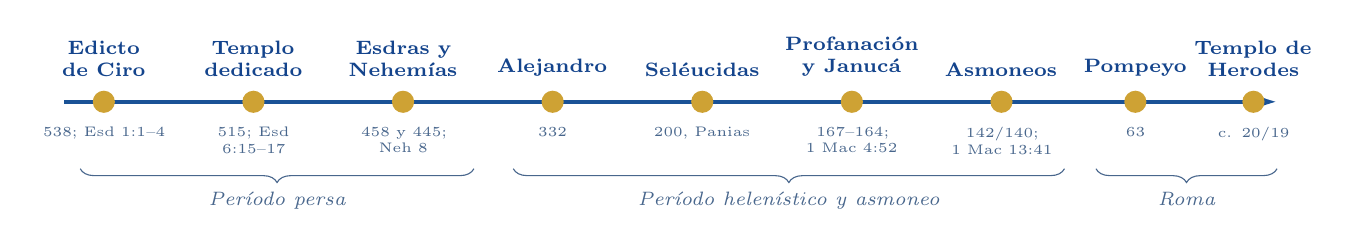
\begin{tikzpicture}[x=1cm,y=1cm]
\draw[line width=1.6pt,cafe,-{Latex[length=3mm]}] (0,0) -- (15.4,0);
\foreach \x/\t/\b in {0.5/{Edicto de Ciro}/{538; Esd 1:1--4},
                      2.4/{Templo dedicado}/{515; Esd 6:15--17},
                      4.3/{Esdras y Nehemías}/{458 y 445; Neh 8},
                      6.2/{Alejandro}/{332},
                      8.1/{Seléucidas}/{200, Panias},
                      10.0/{Profanación y Janucá}/{167--164; 1~Mac 4:52},
                      11.9/{Asmoneos}/{142/140; 1~Mac 13:41},
                      13.6/{Pompeyo}/{63},
                      15.1/{Templo de Herodes}/{c. 20/19}}{
  \fill[oro] (\x,0) circle (4pt);
  \node[above,font=\scriptsize\bfseries,text=ladrillo,text width=1.7cm,align=center] at (\x,0.2) {\t};
  \node[below,font=\tiny,text=sepia,text width=1.7cm,align=center] at (\x,-0.2) {\b};}
\draw[decorate,decoration={brace,amplitude=5pt,mirror},sepia] (0.2,-0.85) -- (5.2,-0.85) node[midway,below=5pt,font=\scriptsize\itshape]{Período persa};
\draw[decorate,decoration={brace,amplitude=5pt,mirror},sepia] (5.7,-0.85) -- (12.7,-0.85) node[midway,below=5pt,font=\scriptsize\itshape]{Período helenístico y asmoneo};
\draw[decorate,decoration={brace,amplitude=5pt,mirror},sepia] (13.1,-0.85) -- (15.4,-0.85) node[midway,below=5pt,font=\scriptsize\itshape]{Roma};
\end{tikzpicture}\\[2pt]
{\footnotesize\color{sepia}\textit{Nota.} Elaboración propia. Fechas a.\,e.\,c.; varias están en debate (véase el texto).}
\end{center}

\section{Contexto histórico y arqueológico}

El \textbf{Cilindro de Ciro}, hallado en Babilonia en 1879, es una proclamación en acadio en la que Ciro, elegido de Marduk, dice haber devuelto a sus santuarios los dioses de varias ciudades «al otro lado del Tigris» y haber hecho volver a sus habitantes (Finkel, 2013). Ilustra la política de Esd 1:1--4, pero no menciona a Judá ni a YHWH: es un testimonio paralelo, no el edicto de Esdras (Kuhrt, 1983). Las tablillas de \textbf{Al-Yahudu}, «la ciudad de Judá», documentan entre 572 y 477 a.\,e.\,c. contratos y deudas de deportados con nombres como \emph{Yahu-azar} (Pearce y Wunsch, 2014): los desterrados de Judá conservaron su identidad y echaron raíces, como les pidió Jer 29:5--7, y por eso la mayoría no volvió. En Egipto, la guarnición judía de \textbf{Elefantina} escribió en 407 a.\,e.\,c. al gobernador de Yehud para reconstruir su templo a YHW y mencionó a los «hijos de Sanbalat, gobernador de Samaria» (Porten y Yardeni, 1986), el adversario de Nehemías (Neh 2:10).

\begin{center}\begin{minipage}{0.85\linewidth}\centering
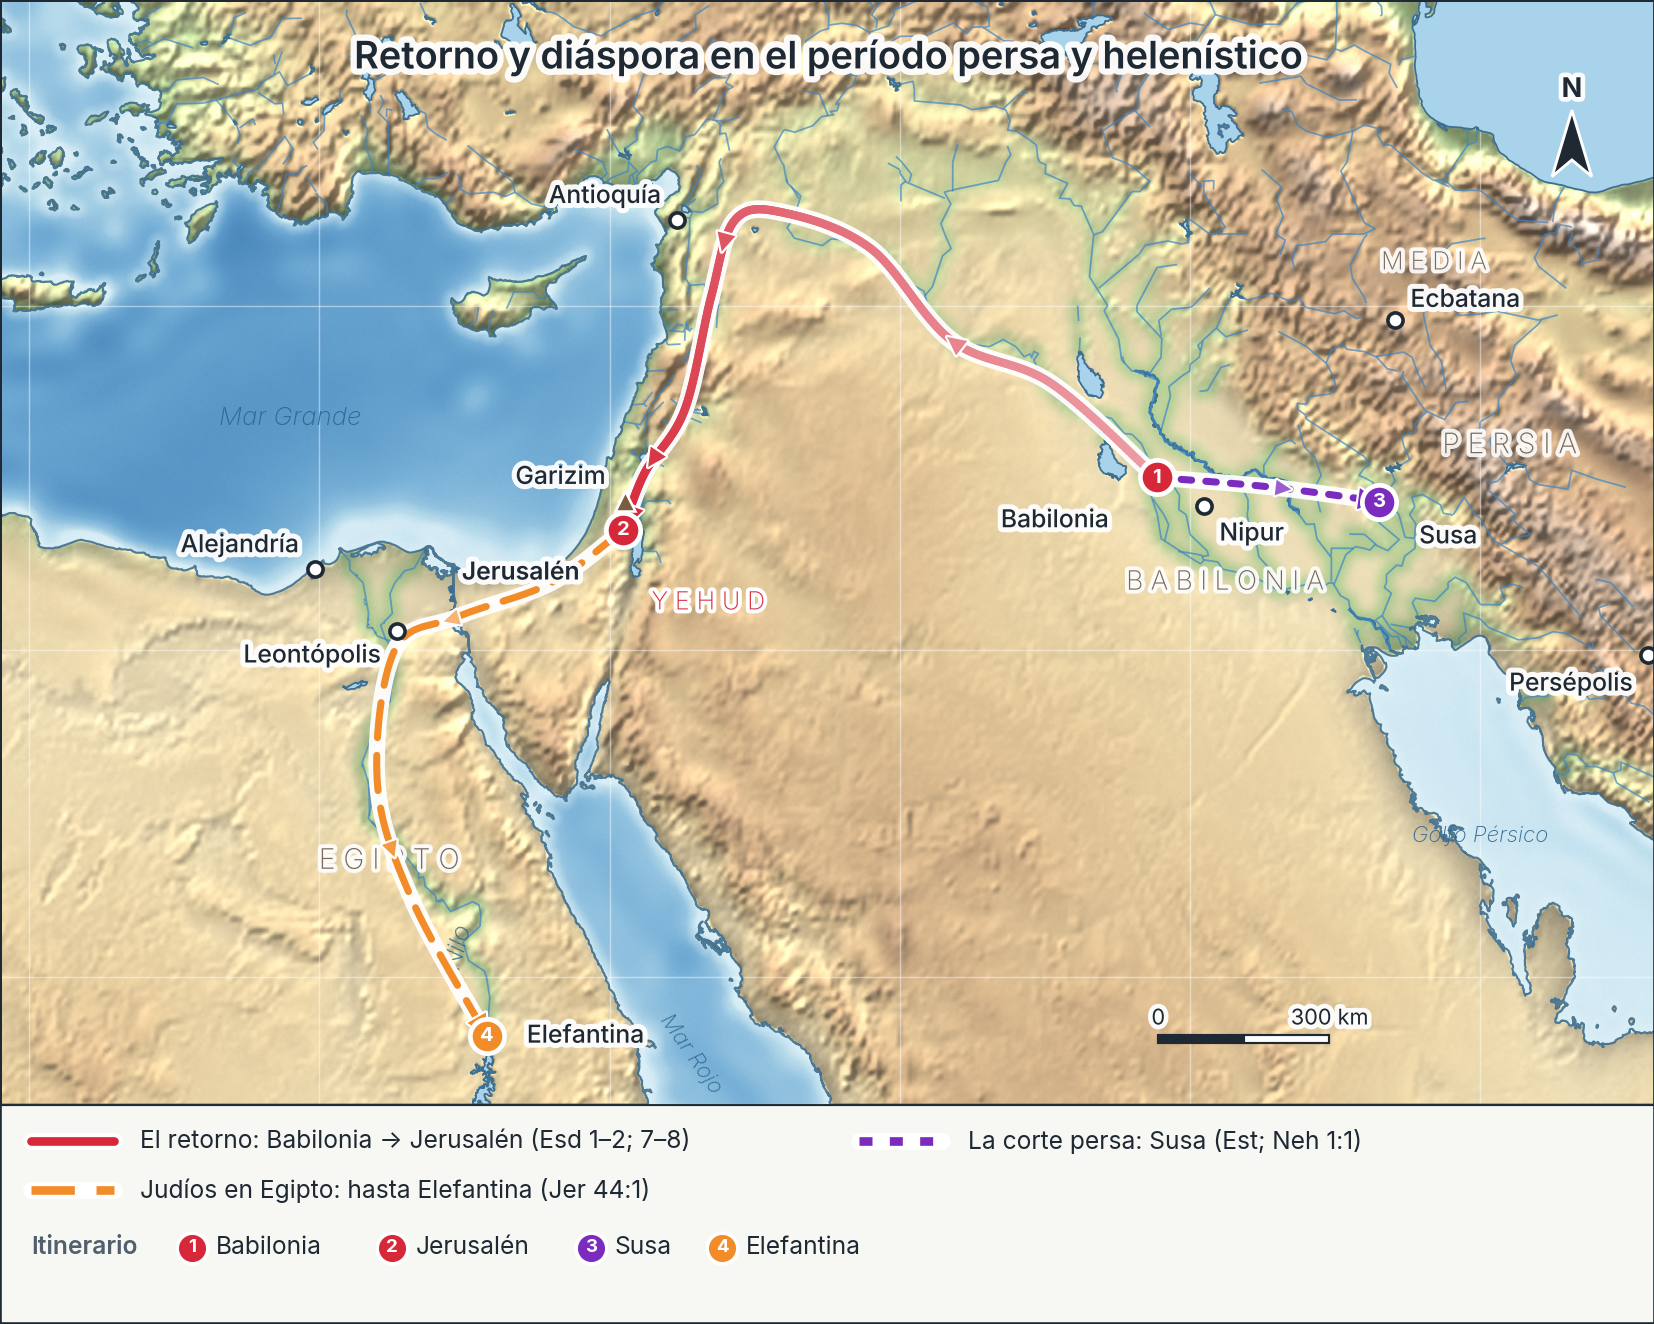
\includegraphics[width=1\linewidth]{mapa_diaspora.png}\\[2pt]
{\footnotesize\color{sepia}\textit{Nota.} Elaboración propia: costas, lagos y ríos GSHHS/WDB y relieve sombreado (Basemap); ubicaciones antiguas aproximadas. }
\end{minipage}\end{center}

La provincia se llamaba \emph{Yehud} (\heb{יְהוּד}; Esd 5:8), y sus impresiones de sello y monedas con las letras \emph{yhd} dibujan una provincia pequeña con administración propia (Lipschits y Vanderhooft, 2011), con una Jerusalén poco poblada, como la de Neh 7:4. Del muro de Nehemías no hay un tramo atribuible con seguridad, pues la torre que Eilat Mazar le asignó es asmonea para Finkelstein (2008). En el monte \textbf{Garizim}, Yitzhak Magen excavó un santuario samaritano de mediados del siglo \textsc{v} a.\,e.\,c., más de un siglo anterior a lo que suponía Josefo (Magen, 2008), trasfondo de Jn 4:20. De los siglos siguientes proceden el gran rollo de Isaías de Qumrán, con diferencias sobre todo ortográficas respecto del Texto Masorético (Ulrich y Flint, 2010), y la inscripción griega del templo herodiano que prohibía a los extranjeros pasar la balaustrada bajo pena de muerte (Josefo, \emph{Guerra} 5.193--194), trasfondo de Ef 2:14.

\section{Desarrollo bíblico}

\subsection{El retorno y la pregunta de quiénes vuelven}
Crónicas termina y Esdras comienza con el mismo edicto, recurso editorial que presenta el retorno como profecía cumplida:
\begin{cita}En el primer año de Ciro, rey de Persia, para que se cumpliera la palabra de YHWH por boca de Jeremías, YHWH despertó el espíritu de Ciro [\ldots]: «[\ldots] Quien haya entre vosotros de todo su pueblo, sea su Dios con él, y suba».\fuente{(Esd 1:1--3; 2 Cr 36:22--23)}\end{cita}
La palabra de Jeremías son los setenta años, e Isaías había llamado a Ciro \heb{מְשִׁיחוֹ}, «su ungido» (Is 45:1), único caso en que un rey extranjero recibe el título de \emph{mashíaj}, que aquí designa una función y no un mesías davídico.

Quienes responden son «los jefes de las casas paternas de Judá y de Benjamín, los sacerdotes y los levitas» (Esd 1:5), sobre todo el antiguo reino del sur. Pero la lista de Esd 2 se titula «el número de los varones del pueblo de \emph{Israel}», y al dedicar el templo esa comunidad actúa en nombre del pueblo entero:
\hebverso{וצפירי עזין לחטאה על כל ישראל תרי עשר למנין שבטי ישראל}
\begin{cita}Y como ofrenda por el pecado por todo Israel, doce machos cabríos, conforme al número de las tribus de Israel.\fuente{(Esd 6:17, arameo)}\end{cita}
Judá y Benjamín no pretenden ser todo Israel, pero al ofrecer por las \emph{doce} tribus declaran vigente la promesa a las ausentes. Según 1~Cr 9:3 vivían además en Jerusalén hijos «de Efraín y de Manasés», aunque el paralelo de Neh 11 solo nombra a Judá y Benjamín y la Biblia no afirma que las diez tribus volvieran como tales. En esos años \heb{יְהוּדִי} (\emph{yehudí}), «de Judá», pierde su sentido tribal, y Mardoqueo es «un judío [\ldots] benjaminita» (Est 2:5). Más dolorosa es la ruptura con los vecinos del norte, que sacrificaban a YHWH «desde los días de Esar-hadón» (Esd 4:2) y a quienes Zorobabel rechaza. Probablemente eran una población mixta de israelitas del antiguo reino del norte no deportados y colonos extranjeros (Crown, 1989), y el conflicto quedó como una herida dentro de la casa de Jacob que el Nuevo Testamento retomará (Jn 4; Hch 8:5--25).

\subsection{Hageo y Zacarías: la gloria postrera y las dos casas}
En 520 a.\,e.\,c. Hageo promete que «mayor será la gloria de esta casa postrera que la de la primera» (Hag 2:9), cuando venga \heb{חֶמְדַּת כָּל־הַגּוֹיִם}, «lo deseable de todas las naciones» (Hag 2:7), que la mayoría entiende como los tesoros de las naciones y la Vulgata tradujo como «el deseado». Al poner a Zorobabel «como anillo de sellar» (Hag 2:23) invierte Jer 22:24: apartada del trono, la línea davídica sigue elegida, aunque Zorobabel nunca reinó.

Zacarías pregunta «¿hasta cuándo no tendrás piedad de Jerusalén?» (Zac 1:12) y responde que muchas naciones se unirán a YHWH sin que Judá deje de ser «su porción en la tierra santa» (Zac 2:10--12 [2:14--16]). Ya consumado el retorno, sigue nombrando a las dos casas: «como fuisteis maldición entre las naciones, \emph{oh casa de Judá y casa de Israel}, así os salvaré y seréis bendición» (Zac 8:13; cf. 10:6, «la casa de José»). La restauración incluye, pues, al reino del norte disperso. Anuncia además a un rey «humilde (\heb{עָנִי}), y cabalgando sobre un asno» (Zac 9:9) y un día en que la casa de David «mirará a mí, a quien traspasaron» (Zac 12:10), texto que Juan aplica a la cruz (Jn 19:37) y que muchos vinculan con Ro 11:26.

\subsection{Ester, Esdras y Nehemías}
En Susa, Amán describe a Israel como «un pueblo esparcido y dividido entre los pueblos» (Est 3:8). De su liberación nace Purim, y el libro, que en hebreo no nombra a Dios, termina con gentiles que «se hacían judíos» (\heb{מִתְיַהֲדִים}, Est 8:17). En Jerusalén, Esdras «había preparado su corazón para inquirir la ley de YHWH y para cumplirla, y para enseñar en Israel» (Esd 7:10); el verbo \heb{לִדְרוֹשׁ} es el mismo del que vendrá \emph{midrash}. Nehemías reconstruye los muros pese a Sanbalat (Neh 6:15), y el centro de ambos libros es la lectura pública de la Torá, cuando los levitas «leían en el libro de la ley de Dios con claridad, y ponían el sentido, de modo que entendían la lectura» (Neh 8:8). Siguen la confesión de Neh 9 y un pacto firmado (\heb{אֲמָנָה}, Neh 9:38 [10:1]): un pueblo se reconstituye en torno a un libro.

\subsection{Malaquías: el Dios que no cambia}
Malaquías habla a una comunidad acostumbrada a su templo. Afirma que el nombre de Dios es grande «entre las naciones» (Mal 1:11), anuncia que «vendrá súbitamente a su templo el Señor a quien vosotros buscáis» (Mal 3:1) y da la razón de que este pueblo siga existiendo:
\hebverso{כִּי אֲנִי יְהוָה לֹא שָׁנִיתִי וְאַתֶּם בְּנֵי־יַעֲקֹב לֹא כְלִיתֶם}
\begin{cita}Porque yo, YHWH, no cambio; por eso vosotros, hijos de Jacob, no habéis sido consumidos.\fuente{(Mal 3:6)}\end{cita}
Es, en otra clave, lo que Pablo dirá del llamamiento irrevocable (Ro 11:29). El canon de los profetas se cierra con la promesa de Elías, que «hará volver el corazón de los padres hacia los hijos» (Mal 4:5--6 [3:23--24]).

\subsection{Los «cuatrocientos años de silencio»}
La expresión es una convención cristiana para el tiempo entre Malaquías y Juan el Bautista. No hubo profeta canónico, y la literatura judía lo reconoce, pero aquellos siglos fueron los más agitados del Segundo Templo. Tras el final del dominio \emph{persa}, Alejandro tomó la costa en 332, y Judea pasó a los Ptolomeos y, desde 200, a los Seléucidas, guerras que Dn 11 describe como las del «rey del sur» y el «rey del norte». En Alejandría, en el siglo \textsc{iii} a.\,e.\,c., la Torá se tradujo al griego; el nombre de «Septuaginta» viene de la leyenda de la \emph{Carta de Aristeas}, y hacia 132 a.\,e.\,c. el nieto de Ben Sirá conocía ya en griego «la ley, los profetas y los demás libros» (Jobes y Silva, 2015).

La crisis \emph{helenística} estalló bajo Antíoco~IV Epífanes (175--164). Jasón compró el sumo sacerdocio y levantó un gimnasio en Jerusalén, en lo que 2~Mac 4:13 llama «auge del helenismo», y como su contrario aparece por primera vez \grc{Ἰουδαϊσμός}, «judaísmo» (2~Mac 2:21). En 167 Antíoco prohibió la circuncisión, el sábado y la Torá, y sobre el altar se erigió «la abominación de la desolación» (\grc{βδέλυγμα ἐρημώσεως}, 1~Mac 1:54), la que Daniel anunciaba al decir «quitarán el continuo sacrificio, y pondrán la abominación desoladora» (Dn 11:31). La tradición sitúa a Daniel en el siglo \textsc{vi}, y la mayoría de la investigación crítica fecha Dn 7--12 hacia 167--164 (Collins, 1993); en cualquier caso, los judíos leyeron su crisis a la luz de ese libro, y Jesús retomó la expresión (Mt 24:15).

La respuesta fue la rebelión \emph{macabea}. Matatías se negó a sacrificar en Modín, y su hijo Judas recuperó Jerusalén: el 25 de kislev de 164 el templo fue purificado y se celebró ocho días la dedicación del altar (1~Mac 4:36--59), origen de la \heb{חֲנֻכָּה} (\emph{janucá}) en que Jesús camina por el pórtico de Salomón (\grc{τὰ ἐγκαίνια}, Jn 10:22). Con los hermanos de Judas se abre la etapa \emph{asmonea}. En 142 «fue quitado el yugo de las naciones de Israel» (1~Mac 13:41), y Simón fue nombrado jefe y sumo sacerdote «hasta que se levante un profeta fiel» (1~Mac 14:41). Sus sucesores se llamaron reyes, y Jerusalén quedó en manos de una dinastía sacerdotal y no davídica. La guerra civil entre los últimos asmoneos abrió la puerta a \emph{Roma}: Pompeyo tomó Jerusalén en 63, y el idumeo Herodes emprendió hacia 20/19 la ampliación del templo (Jn 2:20). La casa postrera superó a la primera en tamaño y belleza; la paz y la gloria que Hageo prometía seguían pendientes.

\section{Israel como nación santa y reino de sacerdotes}

El llamado de Éx 19:5--6 tuvo que vivirse sin rey, casi siempre sin independencia y con la mayoría del pueblo fuera de la tierra. Desde Neh 8 Israel se define por un libro leído y explicado; el sábado se vuelve frontera visible, y bajo Antíoco muchos prefieren morir antes que profanarlo (1~Mac 2:29--38); lejos del templo, la \grc{συναγωγή} reúne cada sábado para leer la ley (Hch 15:21). Allí se acercaron los extranjeros a quienes Is 56:7 prometía «casa de oración para todos los pueblos», prosélitos y «temerosos de Dios» (Hch 10:2) entre los que Pablo hallará su primer auditorio gentil. Zacarías había imaginado la escena:
\begin{cita}En aquellos días, diez hombres de todas las lenguas de las naciones se asirán, sí, se asirán del manto de un judío, diciendo: «Iremos con vosotros, porque hemos oído que Dios está con vosotros».\fuente{(Zac 8:23)}\end{cita}
El \heb{כָּנָף} (\emph{kanaf}) es el borde del manto (Nm 15:38), y las naciones se acercan a Dios tomándose de un israelita fiel, que cumple así la función del sacerdote. La Septuaginta prestó el mismo servicio: a los judíos «les fue confiada la palabra de Dios» (Ro 3:2), y por esa traducción llegó a los gentiles. Los mismos siglos muestran cómo podía quebrarse el llamado. Juan Hircano circuncidó por la fuerza a los idumeos (Josefo, \emph{Ant.} 13.254--258), en las antípodas de Is 56, y la balaustrada del templo acabó como símbolo de la división que, según Pablo, Cristo derribó (\grc{τὸ μεσότοιχον τοῦ φραγμοῦ}, Ef 2:14).

\section{Aporte de la tradición judía}

La Mishná hace pasar la Torá de los profetas a «los hombres de la Gran Asamblea» (\heb{אַנְשֵׁי כְנֶסֶת הַגְּדוֹלָה}), que mandaron «levantad muchos discípulos y haced un cerco a la Torá» (Avot 1:1), y el Talmud atribuye a esa asamblea, que suele relacionarse con Neh 8--10, el orden de la Amidá (Meguilá 17b). Así se reconoce el judaísmo rabínico heredero de Esdras, sin que el dato sea verificable. La misma tradición registra el fin de la profecía: «Cuando murieron Hageo, Zacarías y Malaquías, los últimos profetas, el Espíritu Santo se apartó de Israel; con todo, se servían de la \emph{bat qol}» (Tosefta Sotá 13:3), y Josefo niega que desde Artajerjes hubiera «sucesión exacta de profetas» (\emph{Contra Apión} 1.41). El Nuevo Testamento hará terminar ese silencio con Juan el Bautista (Lc 3:2).

La esperanza de restauración quedó inscrita en la oración diaria. La décima bendición de la Amidá pide:
\hebverso{תְּקַע בְּשׁוֹפָר גָּדוֹל לְחֵרוּתֵנוּ וְשָׂא נֵס לְקַבֵּץ גָּלֻיּוֹתֵינוּ \foreignlanguage{spanish}{[\ldots]} מְקַבֵּץ נִדְחֵי עַמּוֹ יִשְׂרָאֵל}
\begin{cita}Toca el gran shofar por nuestra libertad, alza estandarte para reunir a nuestros desterrados, y reúnenos juntos de los cuatro extremos de la tierra. Bendito eres tú, YHWH, que reúnes a los dispersos de tu pueblo Israel.\fuente{(Amidá, décima bendición; Sacks, 2009)}\end{cita}
La oración entrelaza Is 27:13 e Is 11:12, donde Dios «reunirá los desterrados de \emph{Israel}, y juntará los esparcidos de \emph{Judá}». En Isaías, «Israel» es el reino del norte y «Judá» el del sur; la Amidá habla de «tu pueblo Israel» como pueblo entero. Aunque su redacción es posterior a 70 e.\,c., la esperanza es anterior: Ben Sirá, hacia 180 a.\,e.\,c., ora «reúne a todas las tribus de Jacob» (Eclo 36:10) y espera a Elías «para restablecer las tribus de Jacob» (\grc{καταστῆσαι φυλὰς Ἰακώβ}, Eclo 48:10).

\section{La promesa de restauración}

Los escritos del período no disimulan que el retorno dejó promesas sin cumplir:
\hebverso{הִנֵּה אֲנַחְנוּ הַיּוֹם עֲבָדִים}
\begin{cita}He aquí que hoy somos siervos; en la tierra que diste a nuestros padres [\ldots] he aquí que somos siervos en ella. Y su abundante fruto es para los reyes que has puesto sobre nosotros por nuestros pecados [\ldots].\fuente{(Neh 9:36--37)}\end{cita}
Faltaban el rey davídico, las tribus dispersas por Asiria, la independencia, la gloria visible y el corazón nuevo de Jeremías y Ezequiel. Tobías anuncia un templo reconstruido, «pero no como el primero, hasta que se cumplan los tiempos» (Tob 14:5). Daniel, que confiesa el pecado de «todo Israel, los de cerca y los de lejos» (Dn 9:7), oye que «setenta semanas están determinadas sobre tu pueblo y sobre tu santa ciudad, para terminar la prevaricación [\ldots] y traer la justicia perdurable» (Dn 9:24). Sean cuales sean las lecturas de esas semanas, el retorno de Ciro no puso fin al destierro en sentido pleno, lo que N.~T. Wright (1992) ha llamado, con alcance discutido, un «exilio continuado».

Ninguna profecía moldeó tanto esa espera como la de Isaías, cuyas promesas desbordan lo que se vio en 538:

\begin{center}\small
\renewcommand{\arraystretch}{1.2}
\begin{tabular}{>{\RaggedRight\arraybackslash}p{2.4cm}>{\RaggedRight\arraybackslash}p{6.2cm}>{\RaggedRight\arraybackslash}p{5.3cm}}
\toprule
\textbf{Texto} & \textbf{Promesa} & \textbf{En el Segundo Templo y después}\\
\midrule
Is 11:11--12 & Reunión «por segunda vez» de Israel (norte) y Judá (sur) & Amidá, bendición 10; Eclo 36:10\\
Is 49:5--6 & El Siervo levanta las tribus de Jacob y es luz de las naciones & Eclo 48:10; Lc 2:32; Hch 13:47\\
Is 56:6--8 & Extranjeros en el templo; Dios reúne a los dispersos de Israel «y a otros» & Prosélitos; Mc 11:17\\
Is 60--62 & Las naciones traen a los hijos de Sion; Israel, «sacerdotes de YHWH» (61:6) & Lc 4:18--21; Ro 11:12, 15\\
\bottomrule
\end{tabular}\end{center}

En Is 49:6 el Siervo recibe la misión de «levantar las tribus de Jacob» y otra mayor: «también te di por luz de las naciones (\heb{וּנְתַתִּיךָ לְאוֹר גּוֹיִם})». Levantar a las tribus y alumbrar a las naciones forman una sola obra, y Simeón citará el texto ante el niño Jesús (Lc 2:32). En Is 56:8 el Dios «que reúne a los dispersos de Israel», la fórmula de la Amidá, promete juntar «a otros, además de sus reunidos»: un Israel reunido al que se suman las naciones, figura que Pablo desarrollará con el olivo (Ro 11:17--24). Jeremías, que fijó la fecha del retorno, dejó en el mismo oráculo una promesa que lo excede:
\hebverso{ושבתי את שבותכם וקבצתי אתכם מכל הגוים}
\begin{cita}Cuando se cumplan en Babilonia los setenta años, yo os visitaré [\ldots]. Y seré hallado por vosotros, dice YHWH, y haré volver vuestra cautividad, y os reuniré de todas las naciones y de todos los lugares adonde os arrojé.\fuente{(Jer 29:10, 14)}\end{cita}
Ciro cumplió los setenta años; la reunión «de todas las naciones» quedó como horizonte. Tampoco se sentó un davídico en el trono (Jer 33:17), ni «la casa de Judá» fue con «la casa de Israel» desde la tierra del norte (Jer 3:18). La promesa se concentró en el Hijo de David, y tras Pompeyo los \emph{Salmos de Salomón} piden a Dios que levante a «su rey, el hijo de David», que «distribuirá las tribus sobre la tierra» (Sal Salomón 17:21, 28; R.~B. Wright, 1985).

Lucas abre su evangelio entre quienes aguardaban esa restauración. Simeón «esperaba la consolación de Israel» (\grc{παράκλησιν τοῦ Ἰσραήλ}, Lc 2:25), expresión que remite a Is 40:1, y Ana, de la tribu norteña de Aser, hablaba del niño a los que esperaban «la redención de Jerusalén» (Lc 2:38). Cuando los discípulos preguntan si restaurará el reino a Israel (Hch 1:6), Jesús corrige el calendario sin desmentir la restauración. Pablo, que ante Agripa habla de la esperanza de «nuestras doce tribus» (\grc{τὸ δωδεκάφυλον ἡμῶν}, Hch 26:7), resume estos siglos como «el cumplimiento del tiempo» (\grc{τὸ πλήρωμα τοῦ χρόνου}, Gá 4:4). La misma palabra, \grc{πλήρωμα}, vuelve en Ro 11:12 y 25, y cuando Pablo anuncia que «todo Israel será salvo» lo funda en Is 59:20--21 y 27:9, con eco del nuevo pacto de Jer 31:33--34 (Ro 11:26--27): precisamente las promesas que el retorno de Ciro había dejado abiertas. ONE FOR ISRAEL (2025) lee allí un futuro volverse del pueblo judío a Yeshúa, con los gentiles injertados en un Israel «ampliado, no reemplazado»; el Estudio~8 examinará esa y las demás lecturas.

\section{Conclusión y puente al Estudio 7}

El Segundo Templo enseña que una promesa de Dios puede cumplirse de verdad sin cumplirse todavía del todo. Judá y Benjamín, con sacerdotes, levitas y norteños integrados, volvieron, reconstruyeron la casa y ofrecieron por las doce tribus, en el mundo que dejan ver el Cilindro de Ciro, Al-Yahudu y los sellos de Yehud. Pero el pueblo seguía siendo siervo en su tierra, sin rey davídico y con las tribus del norte dispersas, y por eso Zacarías siguió nombrando a «la casa de Judá y la casa de Israel», Daniel alargó los setenta años y la Amidá pidió cada día la reunión de los desterrados. Entretanto Israel aprendió a ser nación santa sin trono y puso las Escrituras al alcance de las naciones, aunque a veces les cerró la puerta. Sobre la fidelidad del Dios que «no cambia» (Mal 3:6), y sobre las promesas de Isaías y Jeremías que el retorno dejó abiertas, levantará Pablo su afirmación de que el llamamiento de Israel es irrevocable.

Al final del período, en el templo que Herodes estaba ampliando, el sacerdote Zacarías recibe el anuncio de un hijo que irá delante del Señor «con el espíritu y el poder de Elías, para hacer volver los corazones de los padres a los hijos» (Lc 1:17; Mal 4:6 [3:24]). Con esas palabras de Malaquías se rompe el silencio. El Estudio~7, \emph{de Cristo a la destrucción del templo}, seguirá al Mesías en su contexto judío, al remanente que creyó y a la caída del templo en 70 e.\,c.

\section*{Preguntas para la reflexión}\markboth{Preguntas para la reflexión}{}
\begin{enumerate}
\item La comunidad que volvió era sobre todo de Judá y Benjamín, pero ofreció doce machos cabríos «por todo Israel» (Esd 6:17). ¿Qué enseña este gesto sobre la relación entre un remanente y el pueblo entero (Ro 11:5, 16)?
\item Nehemías ora «hoy somos siervos» en plena restauración (Neh 9:36). ¿Cómo distinguir entre un cumplimiento real y un cumplimiento pleno de las promesas de Dios?
\item Zac 8:23 imagina a las naciones tomadas del manto de un judío. ¿Qué actitudes de Israel favorecían esa escena y cuáles la impedían? ¿Qué dice esto a los creyentes de las naciones (Ro 11:18)?
\end{enumerate}

\section*{Glosario}\markboth{Glosario}{}
\begin{description}\small
\item[Bat qol] (\heb{בַּת קוֹל}). «Hija de la voz». Voz del cielo que, según la tradición, ocupa el lugar de la profecía después de Malaquías.
\item[Enkainia / Janucá] (\grc{τὰ ἐγκαίνια}; \heb{חֲנֻכָּה}). «Dedicación». Fiesta de la purificación del templo en 164 a.\,e.\,c. (1~Mac 4:59; Jn 10:22).
\item[Mityahadim] (\heb{מִתְיַהֲדִים}). «Se hacían judíos» (Est 8:17). Primera mención bíblica de gentiles que se unen al pueblo judío.
\item[Pleroma] (\grc{πλήρωμα}). Plenitud, cumplimiento. «El cumplimiento del tiempo» (Gá 4:4); clave en Ro 11:12, 25.
\item[Yehud / Yehudí] (\heb{יְהוּד}, \heb{יְהוּדִי}). Provincia persa de Judá; «judío», de Judá y luego de todo el pueblo (Est 2:5).
\end{description}

\section*{Referencias}\markboth{Referencias}{}
\refapa{Bickerman, E.~J. (1988). \emph{The Jews in the Greek age}. Harvard University Press.}
\refapa{\emph{Biblia Hebraica Stuttgartensia} (5.ª ed.). (1997). Deutsche Bibelgesellschaft.}
\refapa{Collins, J.~J. (1993). \emph{Daniel} (Hermeneia). Fortress Press.}
\refapa{Crown, A.~D. (Ed.). (1989). \emph{The Samaritans}. Mohr Siebeck.}
\refapa{Danby, H. (Trad.). (1933). \emph{The Mishnah}. Oxford University Press.}
\refapa{Epstein, I. (Ed.). (1935--1948). \emph{The Babylonian Talmud}. Soncino Press.}
\refapa{Finkel, I. (Ed.). (2013). \emph{The Cyrus Cylinder: The king of Persia's proclamation from ancient Babylon}. I.\,B. Tauris.}
\refapa{Finkelstein, I. (2008). Jerusalem in the Persian (and early Hellenistic) period and the wall of Nehemiah. \emph{Journal for the Study of the Old Testament, 32}(4), 501--520.}
\refapa{Jobes, K.~H., \& Silva, M. (2015). \emph{Invitation to the Septuagint} (2.ª ed.). Baker Academic.}
\refapa{Josefo, F. (1987). \emph{The works of Josephus} (W. Whiston, Trad.). Hendrickson.}
\refapa{Kuhrt, A. (1983). The Cyrus Cylinder and Achaemenid imperial policy. \emph{Journal for the Study of the Old Testament, 8}(25), 83--97.}
\refapa{Lipschits, O., \& Vanderhooft, D.~S. (2011). \emph{The Yehud stamp impressions: A corpus of inscribed impressions from the Persian and Hellenistic periods in Judah}. Eisenbrauns.}
\refapa{Magen, Y. (2008). \emph{Mount Gerizim excavations: Vol. 2. A temple city}. Israel Antiquities Authority.}
\refapa{Neusner, J. (Trad.). (2002). \emph{The Tosefta}. Hendrickson.}
\refapa{\emph{Novum Testamentum Graece} (28.ª ed.). (2012). Deutsche Bibelgesellschaft.}
\refapa{ONE FOR ISRAEL Ministry. (2025, 3 de julio). \emph{What does «all Israel will be saved» mean in Romans 11?} \url{https://www.oneforisrael.org/what-does-all-israel-will-be-saved-mean-in-romans-11/}}
\refapa{Pearce, L.~E., \& Wunsch, C. (2014). \emph{Documents of Judean exiles and West Semitic exiles in Babylonia in the collection of David Sofer} (CUSAS 28). CDL Press.}
\refapa{Porten, B., \& Yardeni, A. (1986). \emph{Textbook of Aramaic documents from ancient Egypt: Vol. 1. Letters}. Hebrew University.}
\refapa{Rahlfs, A., \& Hanhart, R. (Eds.). (2006). \emph{Septuaginta} (ed. rev.). Deutsche Bibelgesellschaft.}
\refapa{Sacks, J. (Trad.). (2009). \emph{The Koren Siddur}. Koren Publishers.}
\refapa{Ulrich, E., \& Flint, P.~W. (2010). \emph{Qumran Cave 1.II: The Isaiah scrolls} (Discoveries in the Judaean Desert 32). Clarendon Press.}
\refapa{Williamson, H.~G.~M. (1985). \emph{Ezra, Nehemiah} (Word Biblical Commentary 16). Word Books.}
\refapa{Wright, N.~T. (1992). \emph{The New Testament and the people of God}. Fortress Press.}
\refapa{Wright, R.~B. (1985). Psalms of Solomon. En J.~H. Charlesworth (Ed.), \emph{The Old Testament pseudepigrapha} (Vol. 2). Doubleday.}
\end{document}
